\documentclass[usenames,dvipsnames,french]{beamer}

\mode<presentation> {

\usetheme{Montpellier}
}

\usepackage{graphicx} % Allows including images
\usepackage[frenchb]{babel}
\usepackage[T1]{fontenc}
\usepackage[utf8]{inputenc}
% \usepackage[demo]{graphicx}
% \usepackage{caption}

\usepackage{subcaption}
% \usepackage{subfig}
% \usepackage{algorithm,algorithmic}
\usepackage{algorithm2e}
\usepackage{listings}
% \usepackage{ntheorem}
\usepackage{booktabs} % Allows the use of \toprule, \midrule and \bottomrule in tables
\setcounter{tocdepth}{2}
\graphicspath{{../../Figures/}}


\DeclareMathOperator*{\argmin}{arg\,min}
\DeclareMathOperator*{\argmax}{arg\,max}
\newtheorem*{proposition}{Proposition}

% exercices comptés
\newcounter{numexos}%Création d'un compteur qui s'appelle numexos
\setcounter{numexos}{0}%initialisation du compteur
\newcommand{\exercice}[1]{%Création d'une macro ayant un paramètre
\addtocounter{numexos}{1}%chaque fois que cette macro est appelée, elle ajoute 1 au compteur numexos
\textcolor{DarkOrchid}{Exercice\,\thenumexos\,:}\,#1%Met en rouge Exercice et la valeur du compteur appelée par \thenumeexos
}
%----------------------------------------------------------------------------------------
%	TITLE PAGE
%----------------------------------------------------------------------------------------

\setbeamertemplate{title page}{
    \centering

    \Large\bfseries
    Machine learning Tek 5: gradient algorithms
    

\begin{figure}[!h]
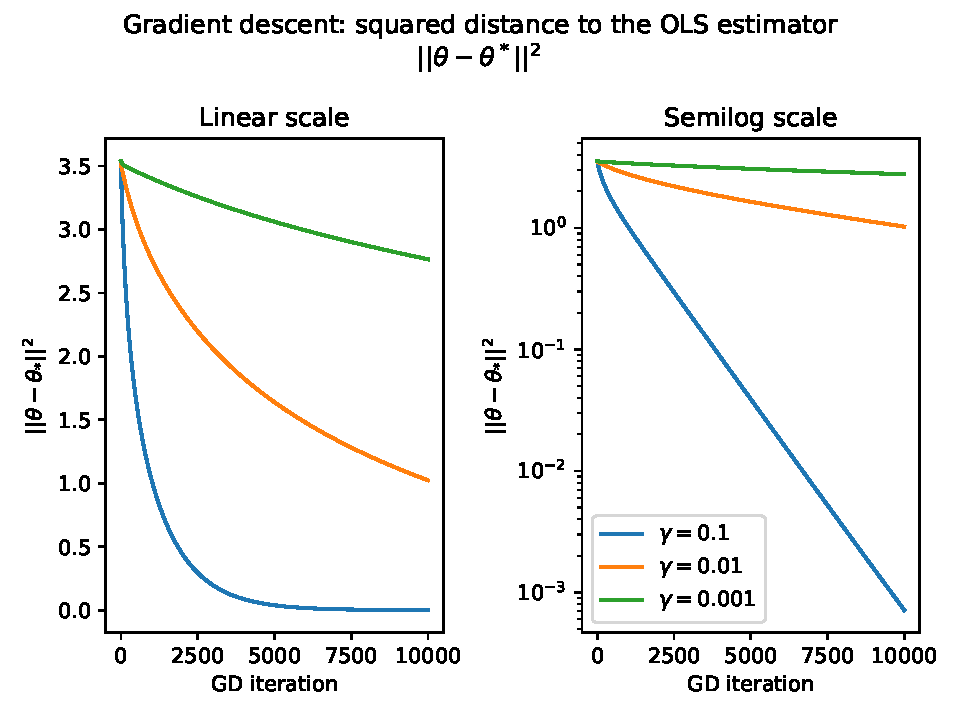
\includegraphics[width=8cm]{Gradient_descent}
\end{figure}

    }
\begin{document}

\frame{\titlepage}

\section{Gradient descent}%
\label{sec:gradient_algorithms}

\subsection{Motivation}%
\label{sub:motivation}

\begin{frame}{Minimization of functions}


    In machine learning, we face \textbf{function minimization problems}. Typically, the function to minimize if the empirical risk on the train set, that will typically depend on a parameter $\theta \in \mathbb{R}^d$.

    \begin{figure}[htpb]
    	\centering
    	
\includegraphics[width=0.5\textwidth]{function_to_minimize_2}
    	\caption{Example of a function to minimize}
    	\label{fig:}
    \end{figure}

\end{frame}

\begin{frame}{Analytic minimum}
   What is the minimum of the function
    \begin{equation}
        f : x \rightarrow (x-1)^2+3.5
    \end{equation}
    And for what value $x$ is it obtained ?
\end{frame}

\begin{frame}{Context}

    In machine learning, we often encounter problems in high dimension, where
    closed-form solutions to the \textbf{empirical risk minimization} problem are \textbf{not} available (e.g. for logistic regression), or
    where even if they are available, the necessary computation time is too
    large (OLS).
    
\end{frame}

\begin{frame}{Context}

    In machine learning, we often encounter problems in high dimension, where closed-form solutions are not avaible, or where even if they are available, the necessary computation time is too large.
    
    \textbf{{Example 1:}} Computing the OLS estimator requires a matrix inversion, which is $ \mathcal{O} (d^3)$.

    \begin{equation}
	\label{def:ols}
	\hat{ \theta}= (X^TX)^{-1}X^Ty
    \end{equation}
\end{frame}

\begin{frame}{Context}

    In machine learning, we often encounter problems in high dimension, where closed-form solutions are not avaible, or where even if they are available, the necessary computation time is too large.
    
    \textbf{{Example 2:}} The cancellation of the gradient of the objective function with logistic loss has no closed-form solution.

\end{frame}

\begin{frame}{Context}


    Instead, we often use \textbf{{iterative}} algorithm such as Gradient descent (GD) or Stochastic gradient descent (SGD). SGD is the standard optimization algorithm for large-scale machine learning.

\end{frame}

\begin{frame}{SGD vs Lapack}

    \begin{figure}[htpb]
        \centering
        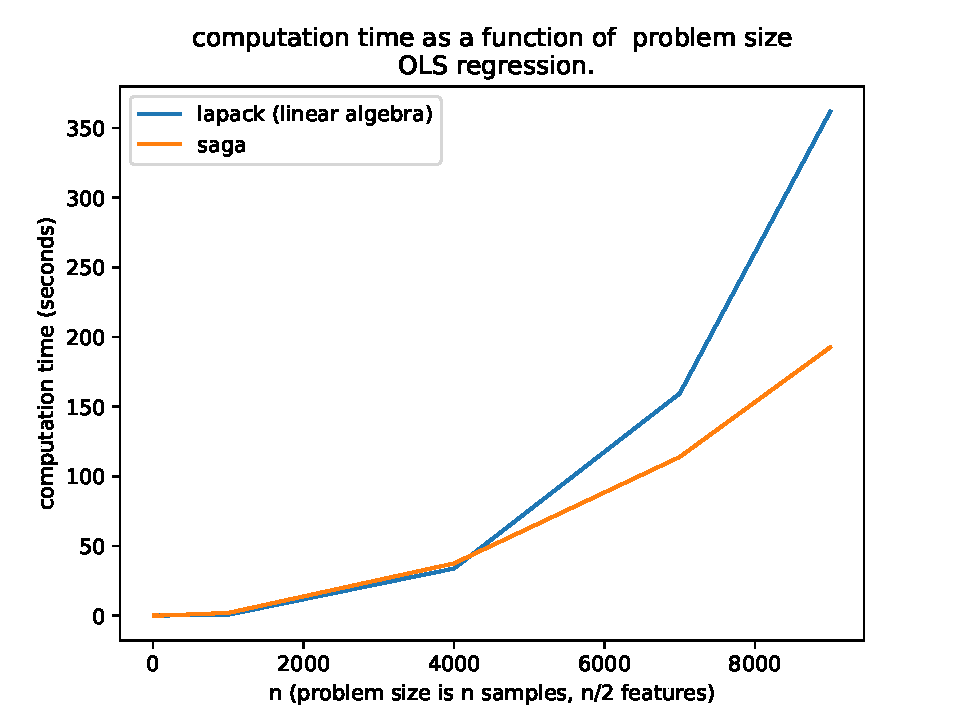
\includegraphics[width=0.8\linewidth]{computation_times}
        \label{fig:computation_times}
    \end{figure}
\end{frame}

\begin{frame}{Derivation and variation}
    \begin{itemize}
        \item In the case a function $ f : \mathbb{R}  \rightarrow
            \mathbb{R}$, we can study its variations by computing its
            derivative $f'$, \textbf{{if it exists}}
        \item If $f'(x)>0$, the function grows around $x$.
        \item If $f'(x)<0$, the function decreases around $x$.
        \item If $x$ is a local extremum, $f'(x)=0$
        \item Is the reciprocal true ?
    \end{itemize}
\end{frame}

\begin{frame}{One dimensional functions}

    If $f: \mathbb{R} \mapsto \mathbb{R} $ is differentiable (dérivable):

    (Landau notation)
    \begin{equation}
        f(a+h) = f(a) + hf'(a) + o(h)
    \end{equation}


    Physicist notation:
    \begin{equation}
        f(a+h) \simeq f(a) + hf'(a)
    \end{equation}
\end{frame}

\begin{frame}{Gradient update}
    In one dimension (the function depends on $x\in \mathbb{R}$): 
            \begin{equation}
                x \leftarrow x-\gamma f'(x)
            \end{equation}
	    \begin{itemize}
		\item $\leftarrow$ means "is substituted by".
	    	\item $\gamma>0$ is a real number called the \textbf{learning rate} (hyperparameter of the algorithm).
	    \end{itemize}
\end{frame}

\begin{frame}{Examples in 1 dimension}
    In the following examples, we use the script \textbf{day\textunderscore 3/gradients/1d\textunderscore function.py}
    \begin{figure}[htpb]
    	\centering
    	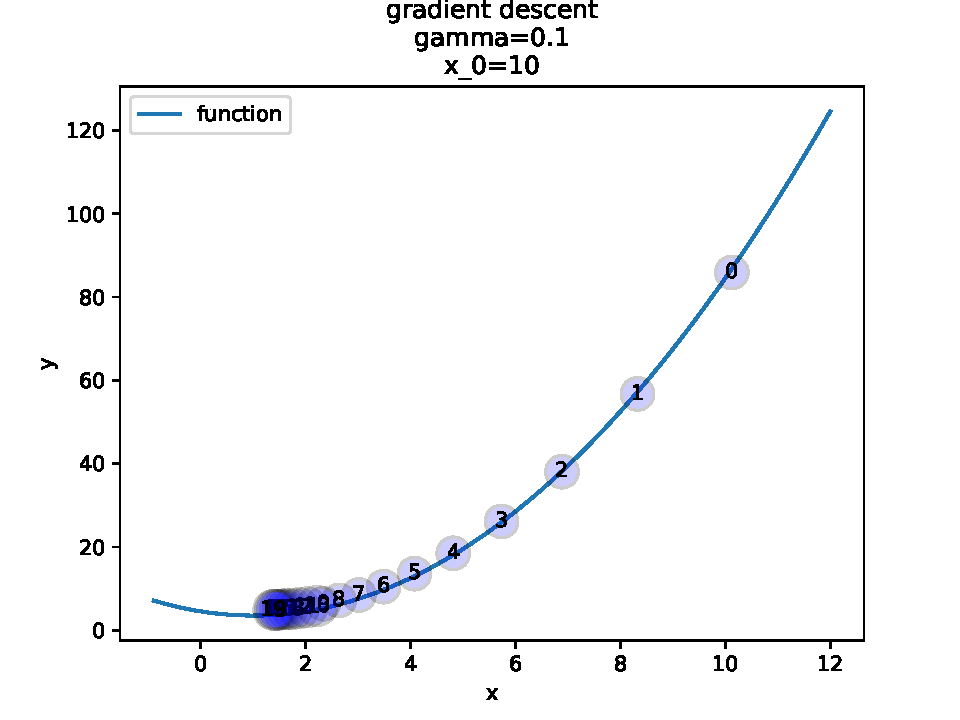
\includegraphics[width=0.8\textwidth]{gd_gamma_0.1_x0_1.0E+01}
    	\label{fig:}
    \end{figure}
\end{frame}


\begin{frame}{Examples in 1 dimension}
    \begin{figure}[htpb]
    	\centering
    	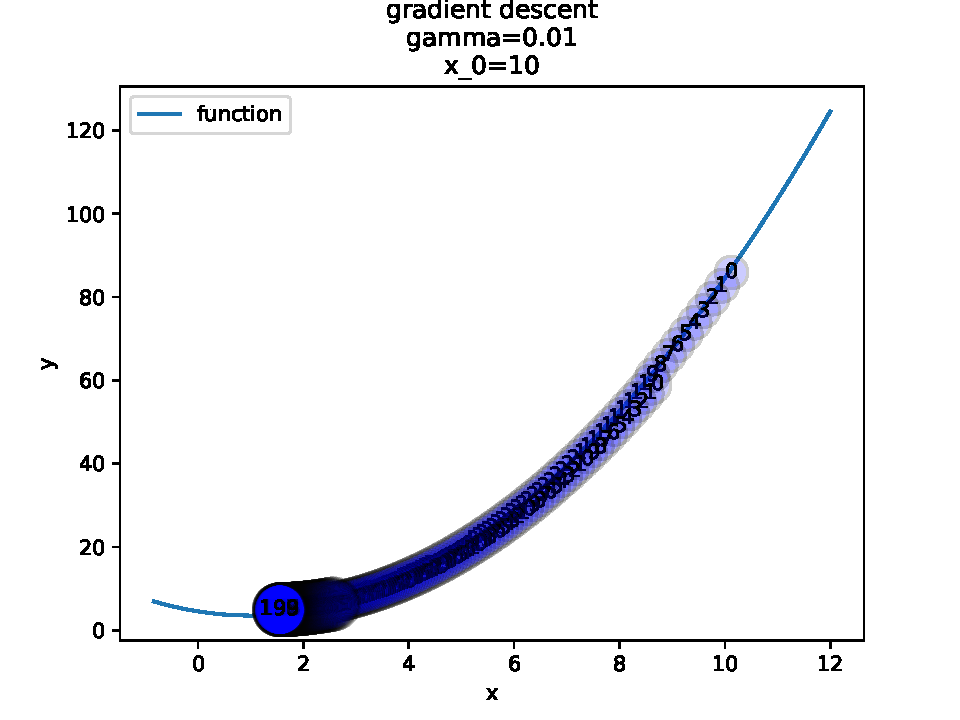
\includegraphics[width=0.8\textwidth]{gd_gamma_0.01_x0_1.0E+01}
    	\label{fig:}
    \end{figure}
\end{frame}


\begin{frame}{Examples in 1 dimension}
    \begin{figure}[htpb]
    	\centering
    	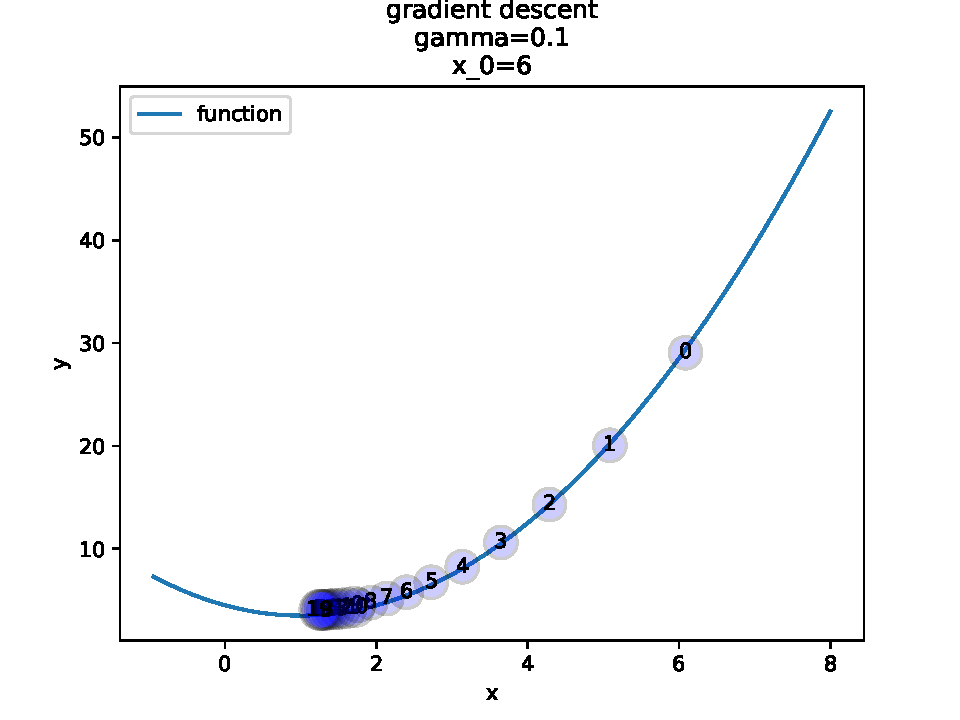
\includegraphics[width=0.8\textwidth]{gd_gamma_0.1_x0_6.0E+00}
    	\label{fig:}
    \end{figure}
\end{frame}


\begin{frame}{Examples in 1 dimension}
    \begin{figure}[htpb]
    	\centering
    	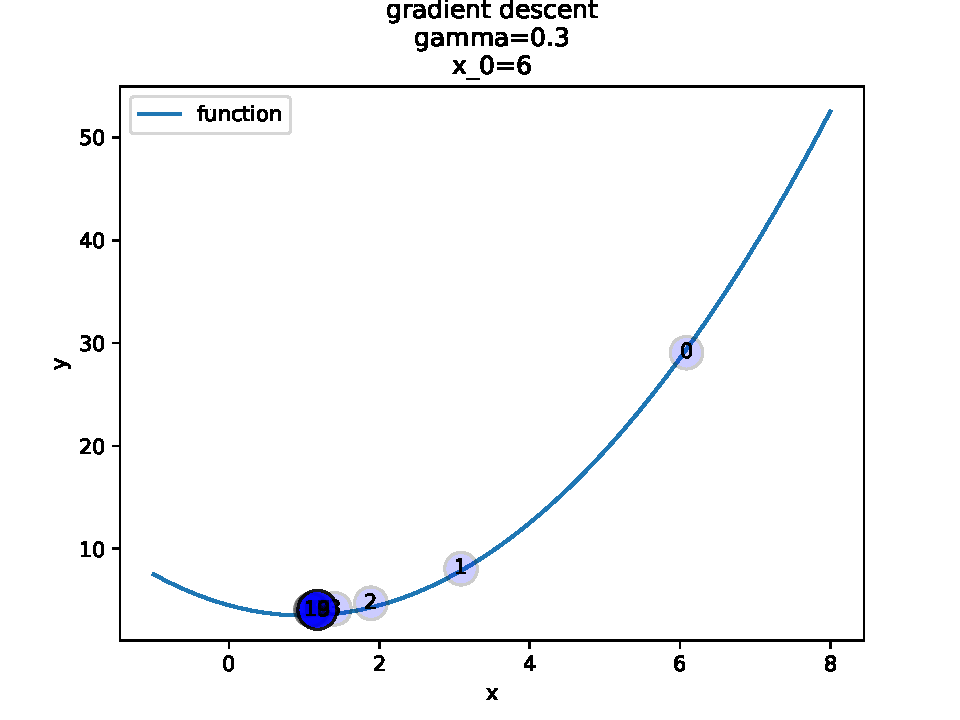
\includegraphics[width=0.8\textwidth]{gd_gamma_0.3_x0_6.0E+00}
    	\label{fig:}
    \end{figure}
\end{frame}


\begin{frame}{Examples in 1 dimension}
    \begin{figure}[htpb]
    	\centering
    	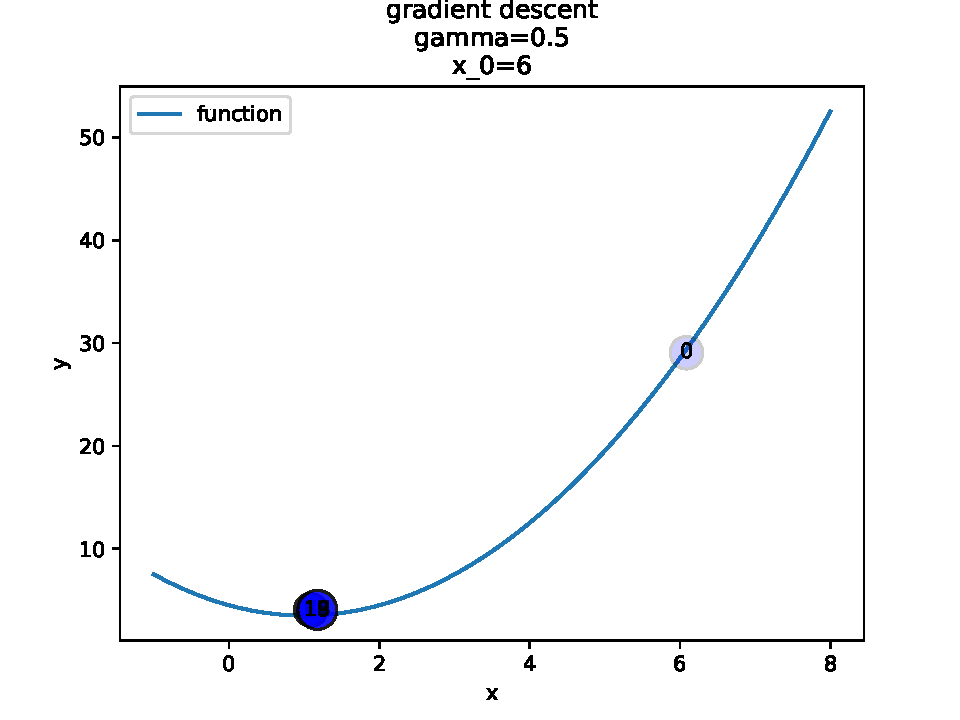
\includegraphics[width=0.8\textwidth]{gd_gamma_0.5_x0_6.0E+00}
    	\label{fig:}
    \end{figure}
\end{frame}


\begin{frame}{Examples in 1 dimension}
    \begin{figure}[htpb]
    	\centering
    	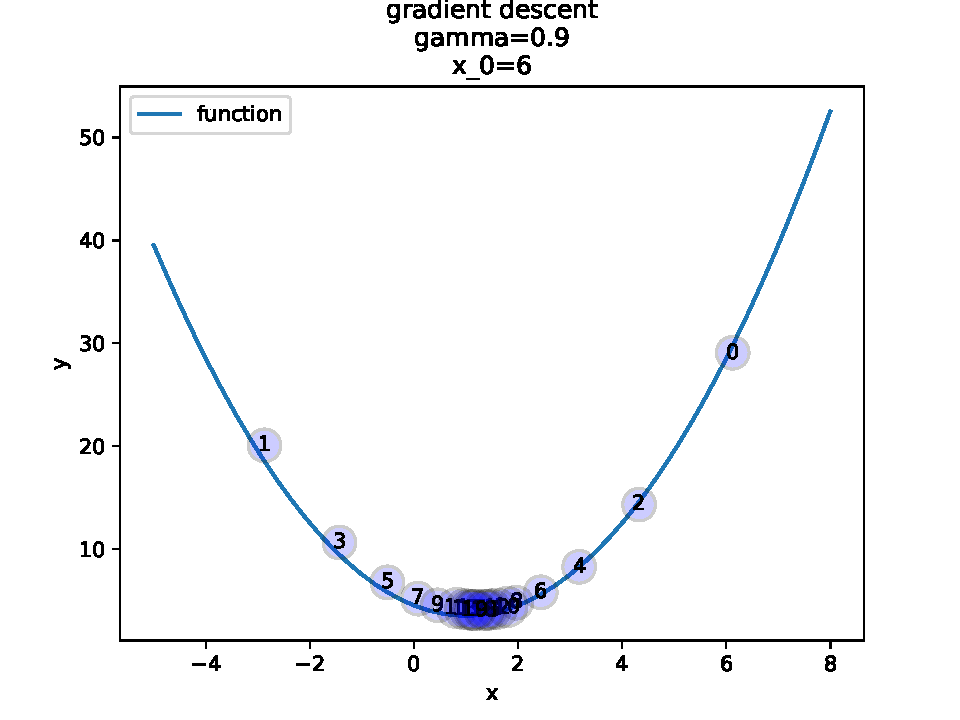
\includegraphics[width=0.8\textwidth]{gd_gamma_0.9_x0_6.0E+00}
    	\label{fig:}
    \end{figure}
\end{frame}


\begin{frame}{Examples in 1 dimension}
    \begin{figure}[htpb]
    	\centering
    	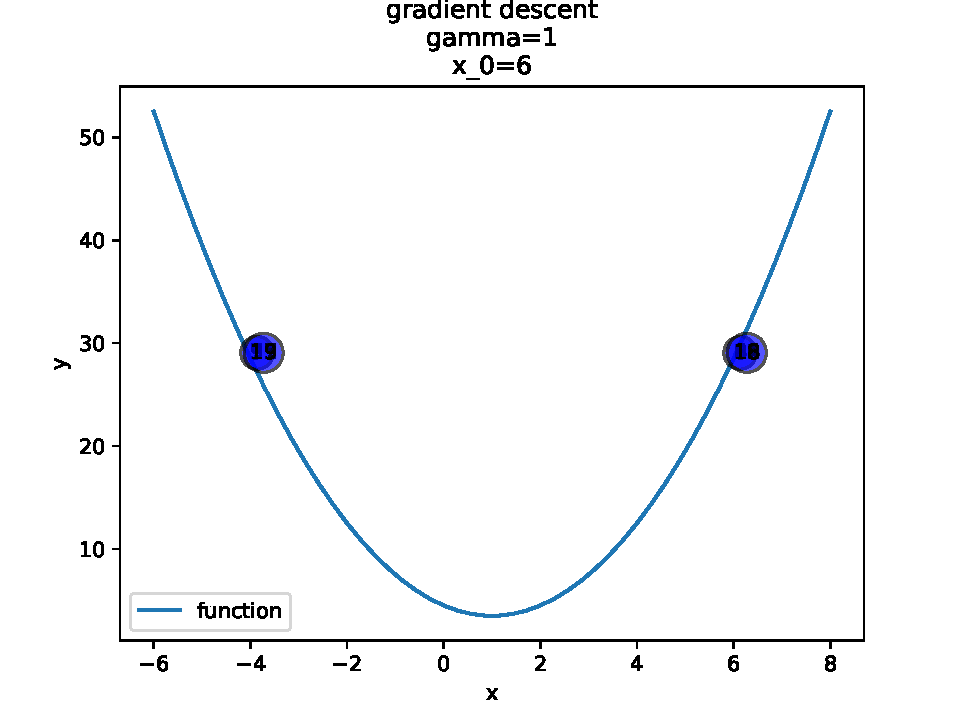
\includegraphics[width=0.8\textwidth]{gd_gamma_1_x0_6.0E+00}
    	\label{fig:}
    \end{figure}
\end{frame}


\begin{frame}{Examples in 1 dimension}
    \begin{figure}[htpb]
    	\centering
    	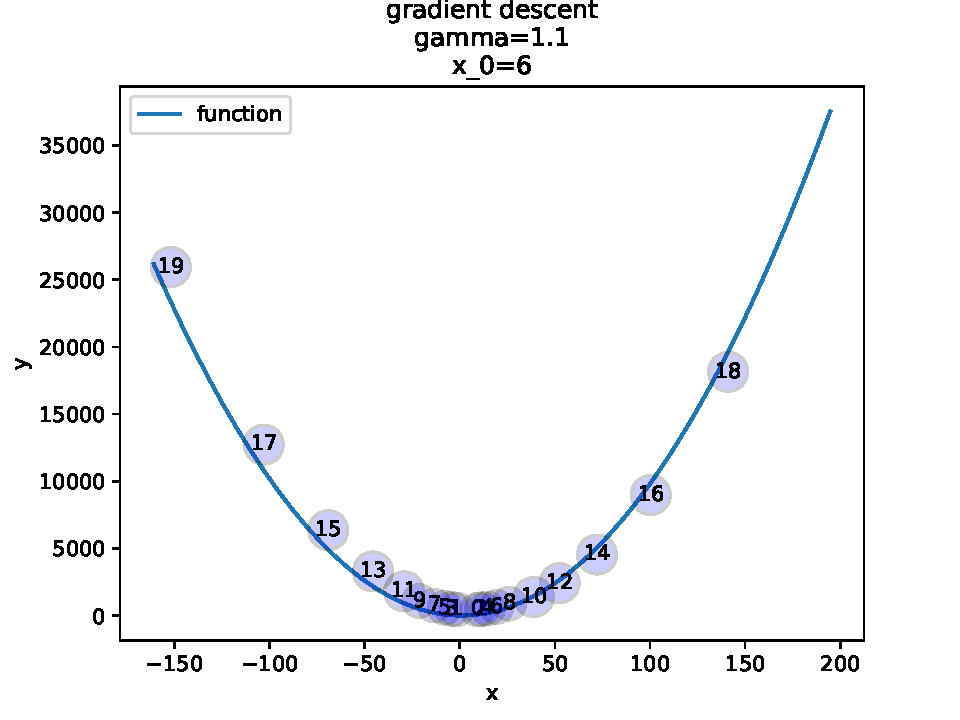
\includegraphics[width=0.8\textwidth]{gd_gamma_1.1_x0_6.0E+00}
    	\label{fig:}
    \end{figure}
\end{frame}


\begin{frame}{Examples in 1 dimension}
    \begin{figure}[htpb]
    	\centering
    	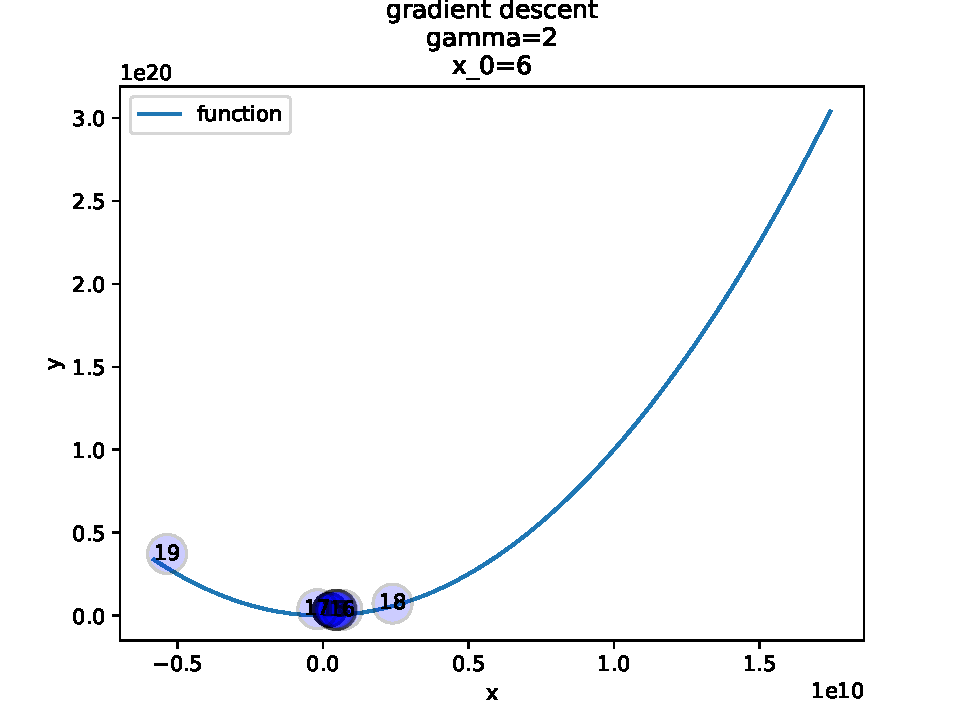
\includegraphics[width=0.8\textwidth]{gd_gamma_2_x0_6.0E+00}
    	\label{fig:}
    \end{figure}
\end{frame}

\begin{frame}{Gradients}
    The \textbf{gradient} is the generalization of the derivative to functions with more than $1$ input variable.

   Example: consider a function $f$ that has $2$ parameters as inputs. If $f$ is differentiable, the gradient writes:
    \begin{equation}
	\nabla f(x,y) = ( \frac{\delta f}{\delta x}(x,y), \frac{\delta f}{\delta y} (x,y))
    \end{equation}

    $\frac{\delta f}{\delta x}(x,y)$ is the \textbf{partial derivative} with respect to $x$, commputed in $(x,y)$. 

\end{frame}

\begin{frame}{Example gradient}

    If
    \begin{equation}
        f(x,y) = x^2 + 3xy + 1
    \end{equation}

    Then
    \begin{equation}
        \forall (x,y)\in \mathbb{R}^2, \nabla f(x,y) = (2x+3y, 3x)
    \end{equation}
\end{frame}

\begin{frame}{Multiple-variable functions}

    If $f: \mathbb{R}^d \mapsto \mathbb{R} $ is differentiable (dérivable):

    (Landau notation)
    \begin{equation}
        f(\theta+h) = f(\theta) + \langle \nabla f(\theta) | h\rangle + o(h)
    \end{equation}


    Physicist notation:
    \begin{equation}
        f(\theta+h) \simeq f(\theta) + \langle \nabla f(\theta) | h\rangle
    \end{equation}

\end{frame}

\begin{frame}{Gradient descent}
\begin{equation}
	\theta\leftarrow \theta-\gamma \nabla f(\theta)
\end{equation}

$\gamma$ must be carefully chosen.

\begin{itemize}
    \item too large $\gamma$: the minimization might not work
    \item too small $\gamma$: the minimization will be too slow
\end{itemize}
\end{frame}



\begin{frame}{Gradient descent algorithm summary:}
    \begin{itemize}
	\item In one dimension (the function depends on $x\in \mathbb{R}$):
            \begin{equation}
                x \leftarrow x-\gamma f'(x)
            \end{equation}
	\item In $d>1$ dimensions (the function depends on $\theta \in \mathbb{R}^d$):
   \begin{equation}
       \theta \leftarrow \theta - \gamma \nabla f(\theta)
   \end{equation} 
		\item $\leftarrow$ means "is substituted by".
		\item $\gamma>0$ is a the \textbf{learning rate}.
    \end{itemize}
\end{frame}


\begin{frame}{Gradient}
    \exercice{\textbf{Implementing the gradient algorithm in $\mathbb{R}^2$}}
\addtocounter{numexos}{-1}

    We will use the algorithm on two functions defined over $\mathbb{R}^2$.
    \begin{figure}[htpb]
        \centering
        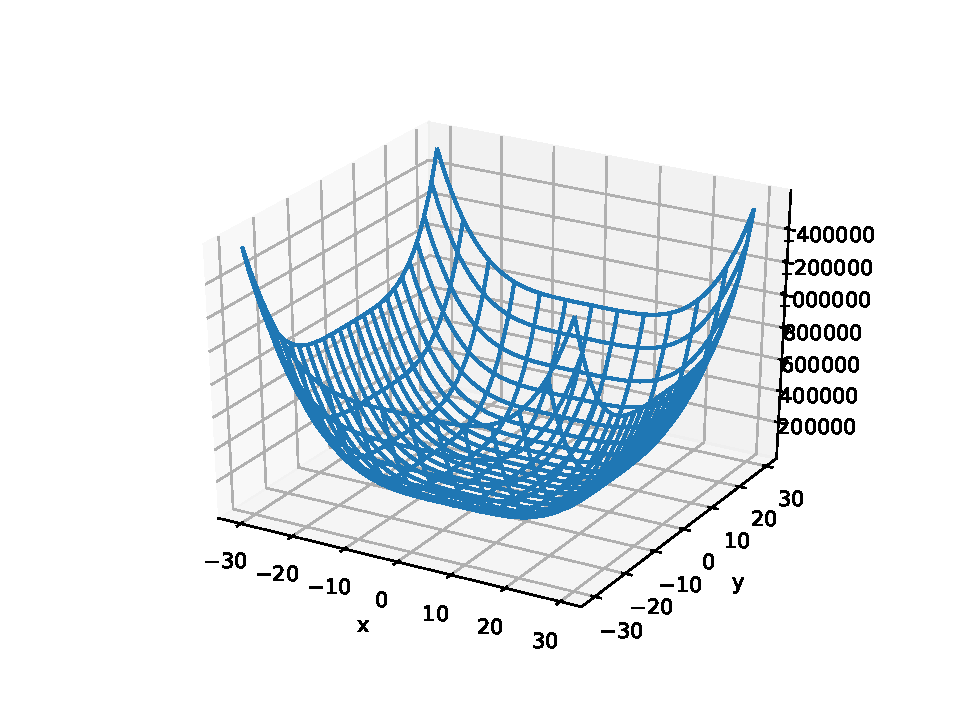
\includegraphics[width=0.75\linewidth]{function_to_minimize}
        \label{fig:function_to_minimize}
    \end{figure}
\end{frame}

\begin{frame}{Gradient}
    \exercice{\textbf{Implementing the gradient algorithm in $\mathbb{R}^2$}}
\addtocounter{numexos}{-1}
    We will use the algorithm on two functions defined over $\mathbb{R}^2$.
    \begin{figure}[htpb]
        \centering
        
\includegraphics[width=0.75\linewidth]{function_to_minimize_2}
        \label{fig:function_to_minimize}
    \end{figure}
\end{frame}

\begin{frame}
    \exercice{\textbf{Implementing the gradient algorithm}}

     In \textbf{{day\textunderscore 3/gradients/}}, use the files \textbf{{gradient\textunderscore algo\textunderscore 1.py}} and \textbf{{gradient\textunderscore algo\textunderscore 2.py}} in order to run the algorithm to find \textbf{{minima}}. Some fixes are required for function 1.
     
     Experiment with all the parameters that you consider relevant (several
     are) to assess their impact on the algorithm.
    \begin{figure}[htpb]
        \centering
        
\includegraphics[width=0.6\linewidth]{function_to_minimize_2}
        \label{fig:function_to_minimize}
    \end{figure}
\end{frame}


\begin{frame}
    \begin{figure}[htpb]
        \centering
        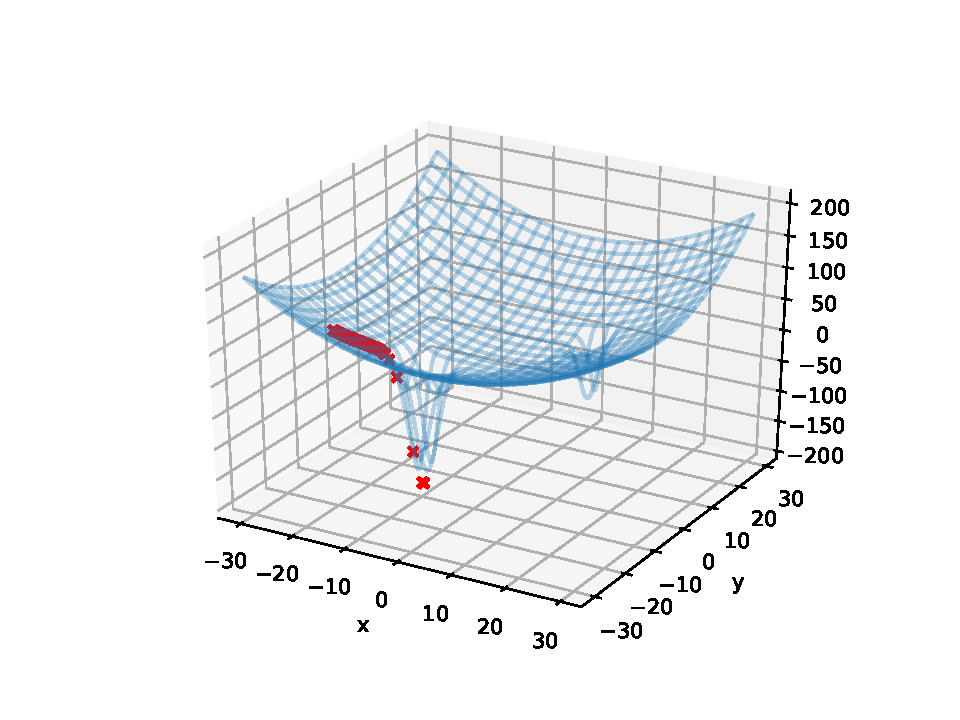
\includegraphics[width=0.94\linewidth]{47500}
        \label{fig:47500}
    \end{figure}
\end{frame}

\begin{frame}
    \begin{figure}[htpb]
        \centering
        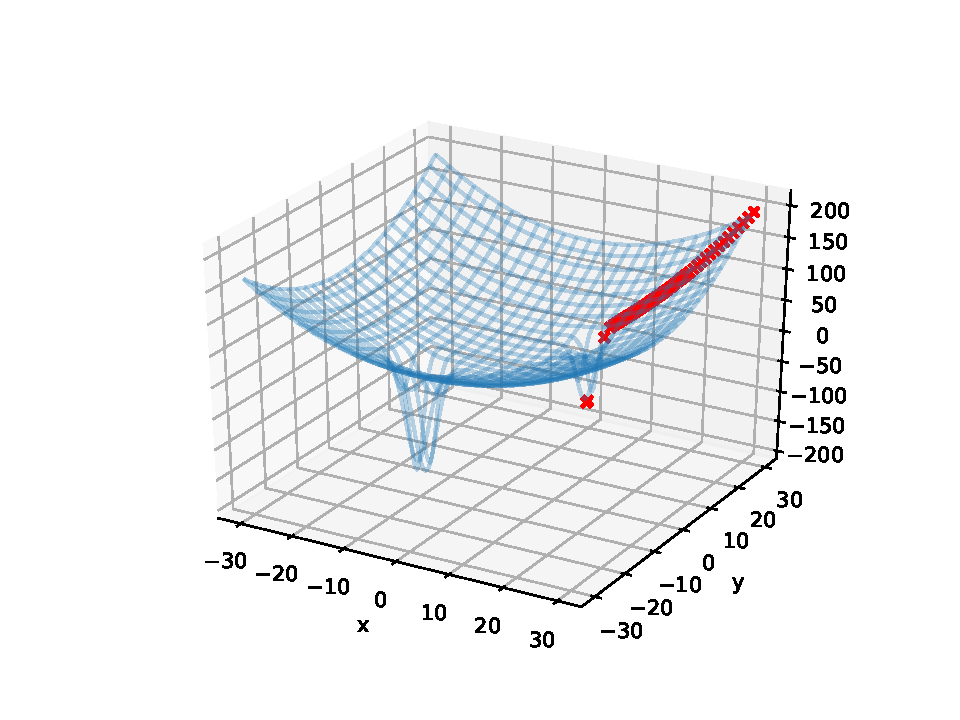
\includegraphics[width=0.94\linewidth]{54000}
        \label{fig:47500}
    \end{figure}
\end{frame}


\begin{frame}
    \begin{figure}[htpb]
        \centering
        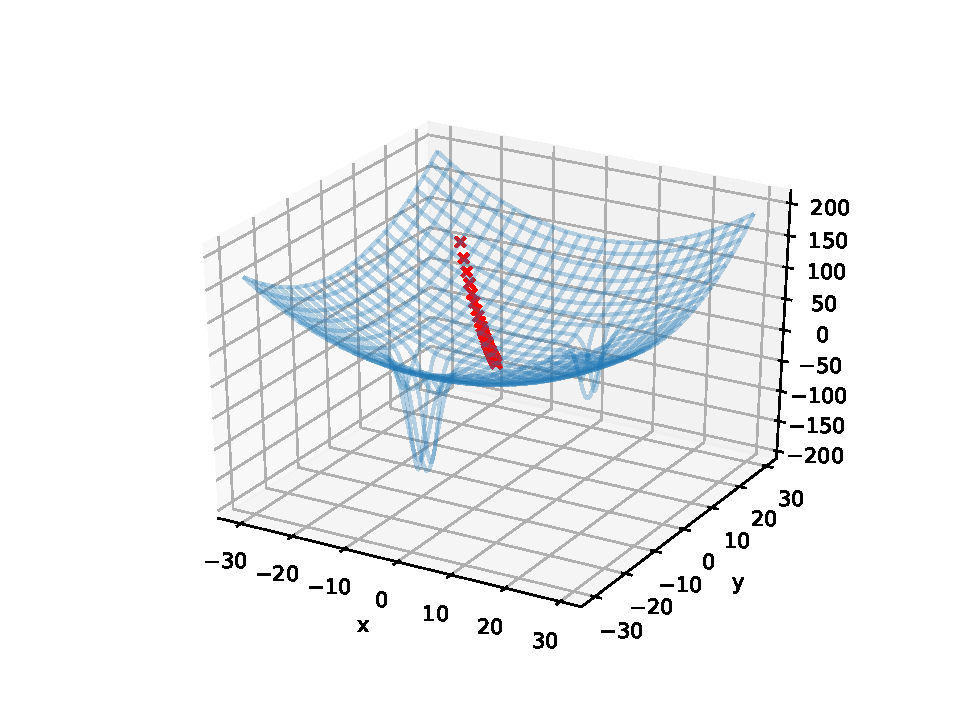
\includegraphics[width=0.94\linewidth]{49500}
        \label{fig:47500}
    \end{figure}
\end{frame}




\begin{frame}{Convergence speed}

    For some problems, it is possible to have garantees on the convergence
    speed of gradient descent. The results will depend on the following properties of the objective function:
    \begin{itemize}
        \item convexity or strong convexity
        \item smoothness (Lipshitz-continuous gradients) or non-smoothness
        \item condition number
    \end{itemize}

\end{frame}

\begin{frame}{Smoothness (Example of theoretical criterion)}
\begin{definition}{Smoothness}

    A differentiable function $f$ with real values is said $L$-smooth if and only if
    \begin{equation*}
	\forall x, y\in \mathbb{R}^d, |f(y)-f(x)-\nabla_xf(y-x)|\leq \frac{L}{2} ||y-x||^2
    \end{equation*}
\end{definition}
\end{frame}



\begin{frame}{}

    \begin{figure}[htpb]
        \centering
        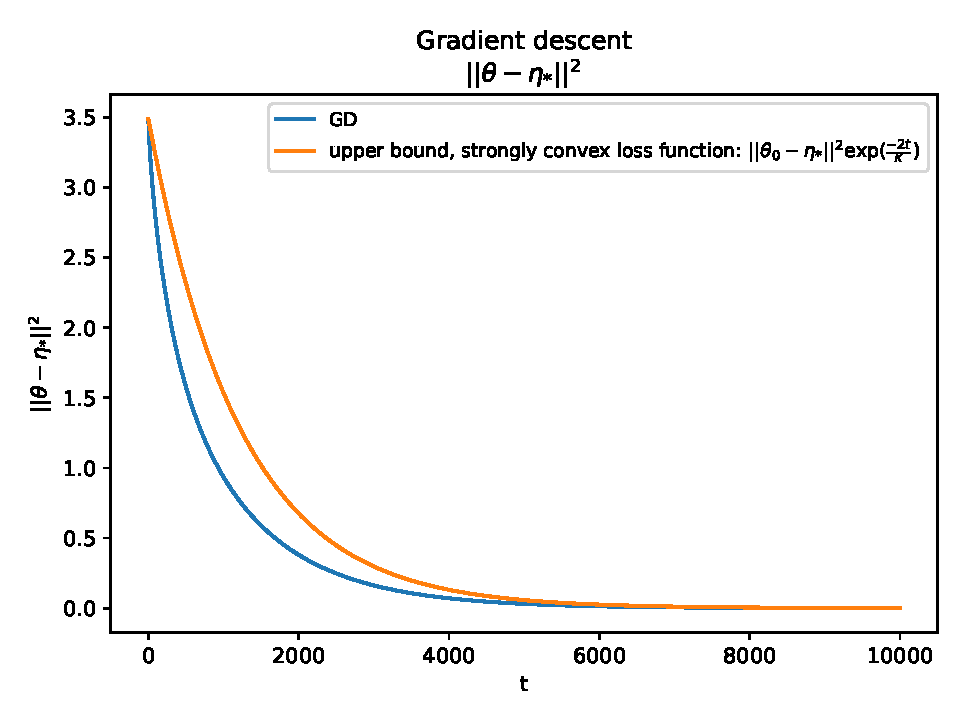
\includegraphics[width=0.8\textwidth]{GD_strongly_convex}
        \label{fig:GD_strongly_convex}
    \end{figure}

\end{frame}

\begin{frame}{}
    \begin{figure}[htpb]
        \centering
        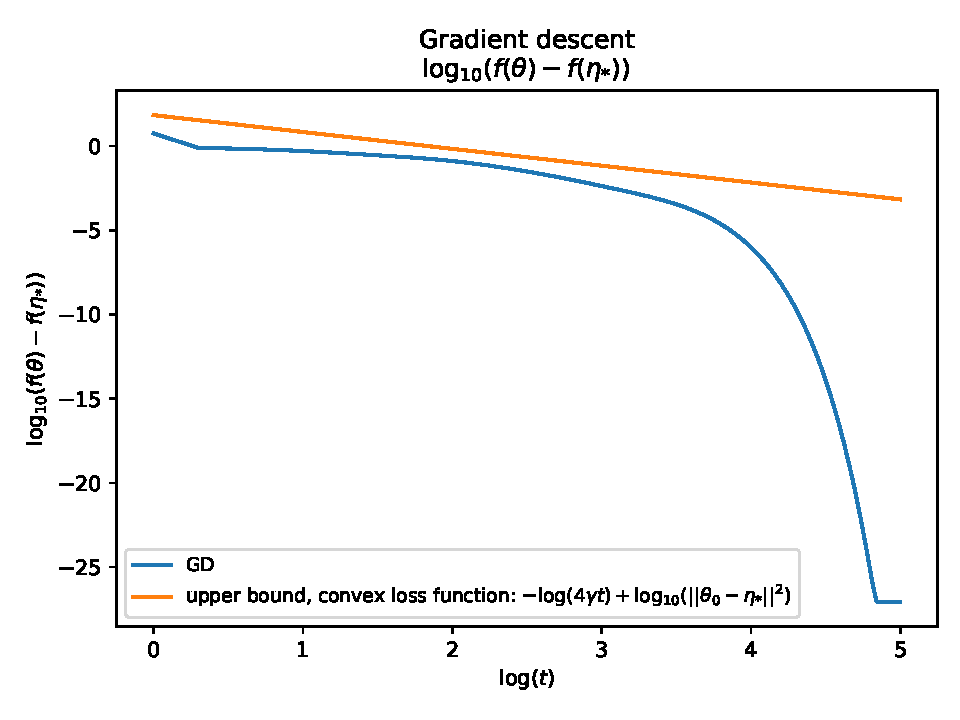
\includegraphics[width=0.8\textwidth]{GD_convex_log}
    \end{figure}

\end{frame}

\begin{frame}{}
    \begin{figure}[htpb]
        \centering
        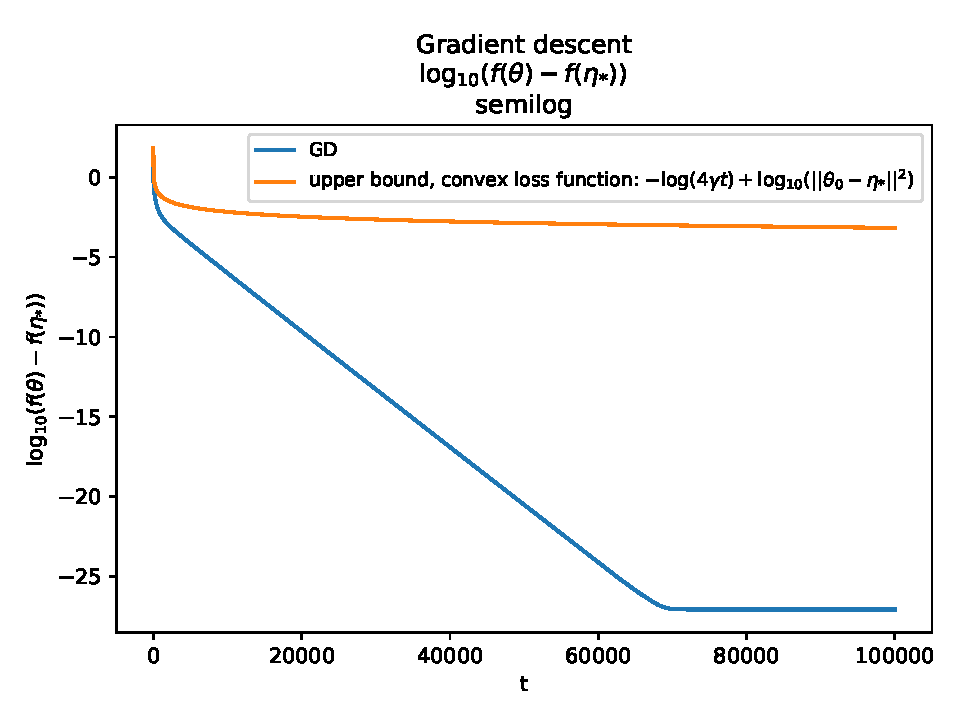
\includegraphics[width=0.8\textwidth]{GD_convex_semilog}
    \end{figure}

\end{frame}

\begin{frame}{Extensions}

    \begin{itemize}
	\item Line search
        \item Nesterov accleration (optimal rates among algorithms that
            linearly combine gradients)
    \end{itemize}
\end{frame}

\begin{frame}{}
    \begin{figure}[htpb]
        \centering
        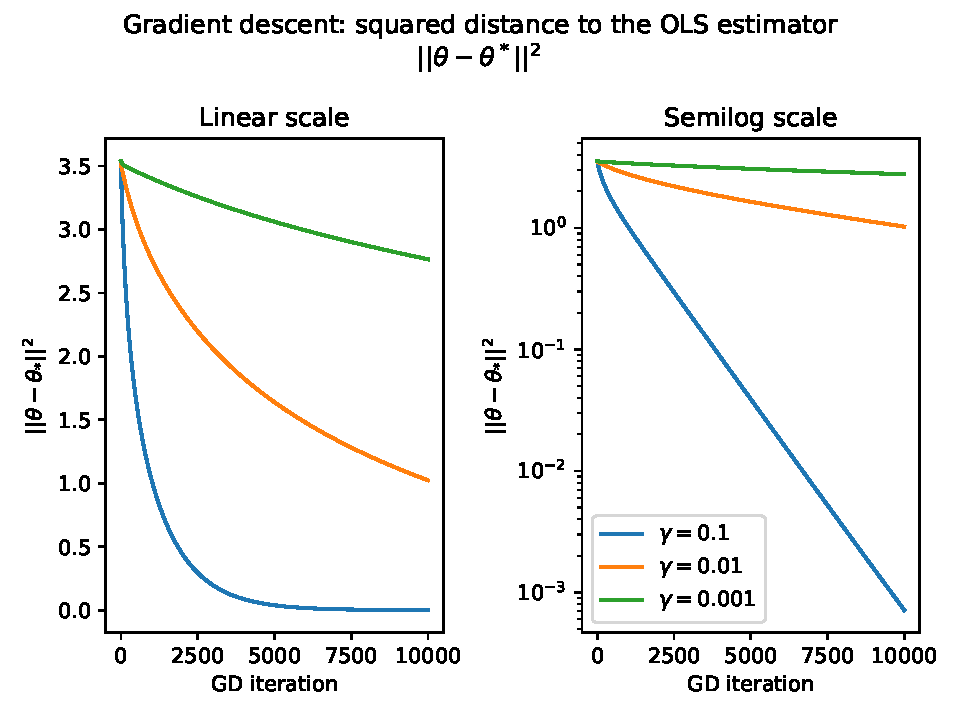
\includegraphics[width=0.8\textwidth]{Gradient_descent}
    \end{figure}

\end{frame}


\section{Stochastic gradient descent}

\begin{frame}{Stochastic gradient descent}
    In machine learning, we often consider an objective function of the form
    \begin{equation}
	f(\theta) = \frac{1}{n} \sum^{n}_{i=1} l(y_i, f_{\theta}(x_i))+\Omega(\theta)
    \end{equation}
    Example with Ridge regression:
    \begin{equation}
	f(\theta) = \frac{1}{n} \sum^{n}_{i=1} ((\theta|x_i)-y_i)^2+\lambda ||\theta||^2
    \end{equation}
    \begin{itemize}
	\item $f_{\theta}(x_i) = (\theta|x_i)$ (dot product)
	\item $l(z, z') = (z-z')^2$
    \end{itemize}
\end{frame}


\begin{frame}{Batch gradient}
    In machine learning, we often consider an objective function of the form
    \begin{equation}
	f(\theta) = \frac{1}{n} \sum^{n}_{i=1} l(y_i, f_{\theta}(x_i))+\Omega(\theta)
    \end{equation}
    Computing the gradient of $f$ requires at least $n$ calculations, and each calculation also has a complexity that depends on the dimension $d$. When $n$ and $d$ are large, this might not be the optimal approachmight not be the optimal approach.
\end{frame}

\subsection{Gradient estimates}%
\label{sub:gradient_estimates}


\begin{frame}{Stochastic gradient descent}
    We consider an objective function of the form
    \begin{equation}
	f(\theta) = \frac{1}{n} \sum^{n}_{i=1} l(y_i, f_{\theta}(x_i))+\Omega(\theta)
    \end{equation}
    Instead of computing the \textbf{{batch gradient}} $\nabla f(\theta)$, we
    will compute the gradient \textbf{with respect to $1$ sample $i$}: 

    \begin{equation}
        u(i, \theta)=\nabla_{\theta}[l(y_i, f_{\theta}(x_i))+\Omega(\theta)]
    \end{equation}

    for a randomly sampled $i\in [1, n]$. $u(i, \theta)$ is an \textbf{estimation} of the full (batch) gradient $\nabla_{\theta}f$.

    Example with Ridge regression:

    \begin{equation}
	\begin{aligned}
		\label{eq:}
	    u(i, \theta)&=\nabla_{\theta}[((\theta|x_i)-y_i)^2+\lambda ||\theta||^2]\\
			&=2((\theta|x_i)-y_i)x_i + 2\lambda\theta
	\end{aligned}
    \end{equation}
    

\end{frame}

\begin{frame}{Tradeoff}

    By replacing the computation of the full gradient (GD) by this estimation
    (SGD):
    \begin{itemize}
        \item we reduce the computation time (divide it by $n$)
        \item but we reduce the precision of the optimization
    \end{itemize}

    To summarize: if $n$ is really large, SGD is often better.


\end{frame}

\begin{frame}{}
    \begin{figure}[htpb]
        \centering
        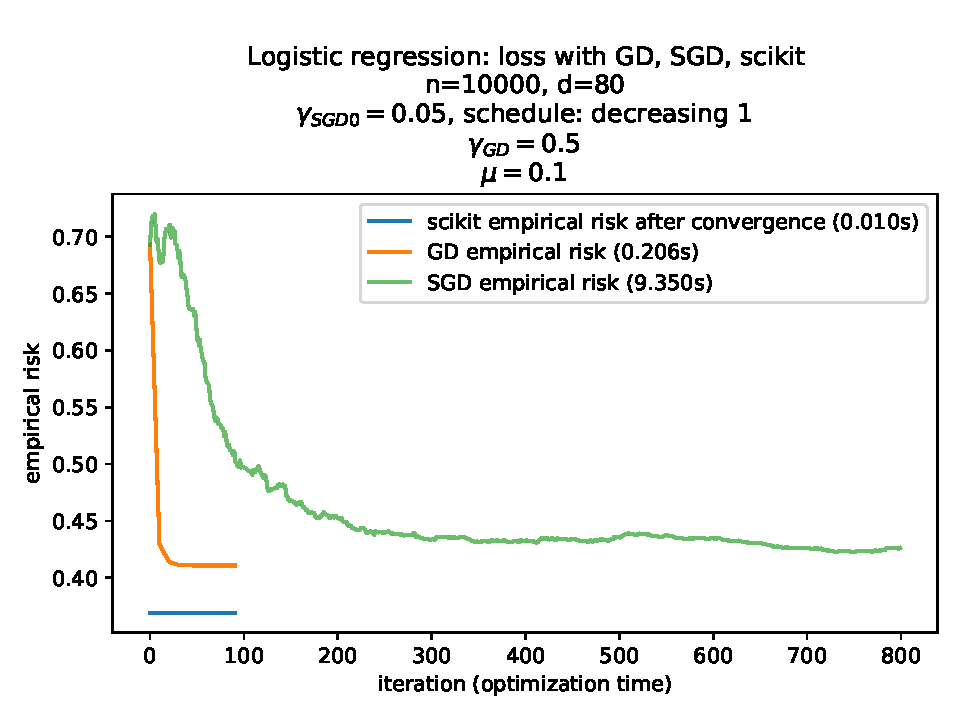
\includegraphics[width=0.8\textwidth]{convergence}
    \end{figure}
\end{frame}

\begin{frame}{}
    \begin{figure}[htpb]
        \centering
        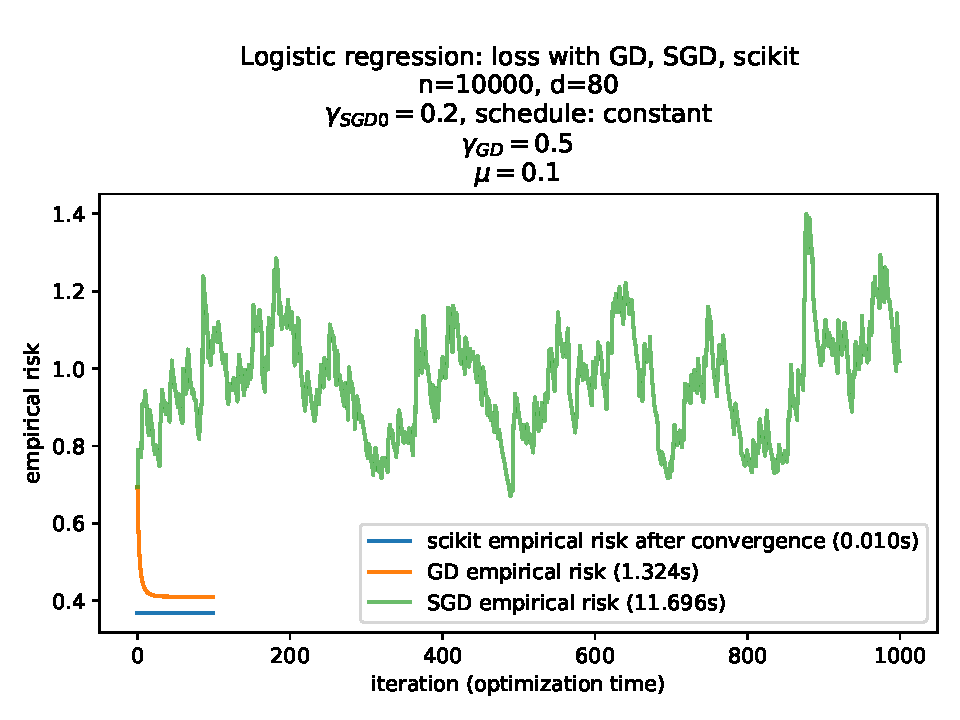
\includegraphics[width=0.8\textwidth]{noconv}
    \end{figure}
\end{frame}


\begin{frame}{}
    \begin{figure}[htpb]
        \centering
        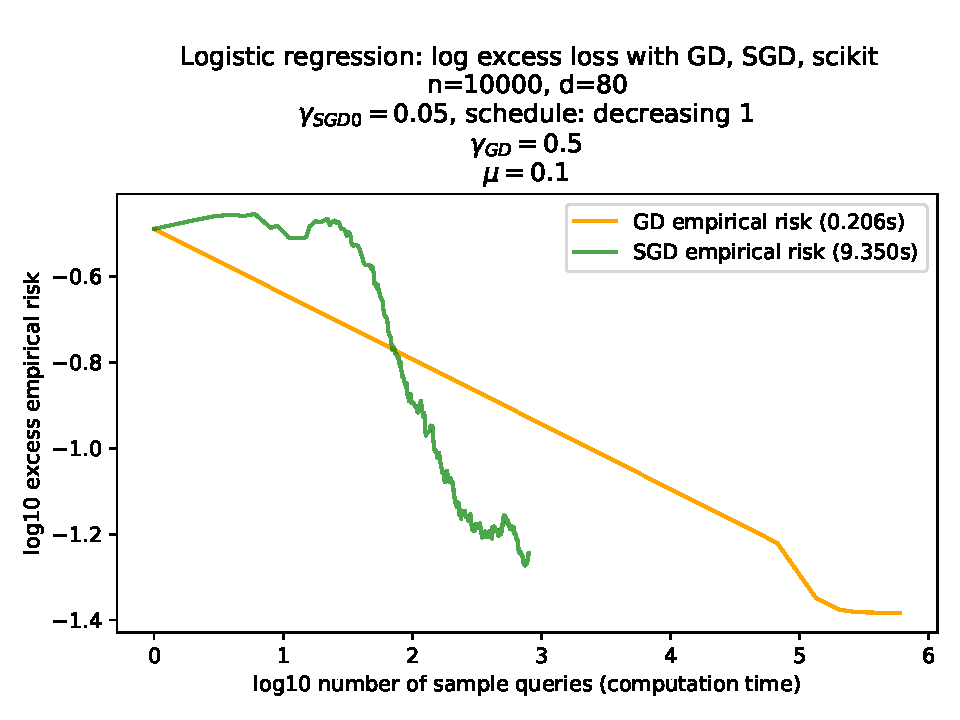
\includegraphics[width=0.8\textwidth]{convergence_nb_queries}
    \end{figure}
\end{frame}

\begin{frame}{Comparison (advanced)}

    The ridge regression problem is smooth and strongly convex.
    
\begin{itemize}
    \item GD has a convergence rate of $\mathcal{O} (\exp( - \frac{t}{\kappa} ))$. To get an error of $\epsilon$, we must have $ t= \mathcal{O} ( \kappa \log \frac{1}{\epsilon} )$. Since each iteration requires $ \mathcal{O} (nd)$ computations, the computation time will be $ \mathcal{O} (\kappa nd\log\frac{1}{\epsilon}) $.
    \item SGD has a convergence rate of $ \mathcal{O} ( \frac{\kappa}{t} )$. To get an error of $\epsilon$, we must have $ t = \mathcal{O}( \frac{\kappa}{\epsilon} ) $. Since each iteration is $ \mathcal{O} (d)$, we have a computation time of $ \mathcal{O} ( \frac{\kappa d}{\epsilon} )$.

\end{itemize}
\end{frame}

\begin{frame}{Comparison (advanced)}
As a consequence:
\begin{itemize}
    \item When $n$ is large and $\epsilon$ not too small, GD will need more computation time to reach error $\epsilon$. An order of magnitude can be obtained by studying the value $\epsilon^*$ such that

	\begin{equation*}
	   \kappa nd \log \frac{1}{\epsilon^*}  = \frac{\kappa d}{\epsilon^*} 
	\end{equation*}

	Which translates to

	\begin{equation*}
	    \epsilon^* \log \epsilon^* = -\frac{1}{n}  
	\end{equation*}
    \item When $\epsilon \rightarrow 0$, GD becomes faster than SGD to reach this precision.
\end{itemize}
\end{frame}

\begin{frame}{Conclusion}
    
For lower precision and large $n$, SGD is a preferable.

    In machine learning, due to the estimation error that is $ \mathcal{O} (
\frac{1}{\sqrt{n} }) $, a very high precision is often not needed 
\end{frame}

\begin{frame}{Minibatch gradient}

    In practical applications, \textbf{minibatches} are very often used. The gradient is computed using a number of samples (instead of $1$), typically $32$, $64$ or more, depending on the available hardware.

\end{frame}

\end{document} 
